\documentclass[10pt]{beamer}
% to hide notes set beamer option
%\documentclass[10pt, handout]{beamer} % exportiere Frames ohne Animation

% template preamble
\usepackage{pgfpages} % Notizen am Rand
\usepackage[ngerman]{babel} % Deutsch

\usetheme[
	subsectionpage=progressbar, 
	progressbar=frametitle, 
	sectionpage=progressbar, 
	block=fill
]{metropolis}

\title{flat-organizer}
\date{\today}
\author{Silas Hoffmann}
\institute{Fachhochschule Wedel}
\titlegraphic{\hfill
\includegraphics[height=1.5cm]{_img/logo_alpha}}


% pdfpages - Einstellungen (Notizen)
%\setbeameroption{hide notes} % Only slides
%\setbeameroption{show only notes} % Only notes
\setbeameroption{show notes on second screen=right} % Both



\begin{document}

\maketitle
  
\section{Projektbeschreibung}
\begin{frame}{Beschreibung des Problems}

Bisher:
\begin{itemize}
\item Große WG immer schwierig zu koordinieren
\item Mitglieder mit zugeteilten Diensten
\item Bisher: Werkzeuge auf diverse Plattformen verteilt
\end{itemize}
\note[item]{Zugeteilte Dienste: Einkauf, Putzen Küche, Klo, Flur, Müll, etc.}

Idee:
\begin{itemize}
\item Eine Plattform für alles
\item Erstes Zwischenprojekt \glqq Einkaufsliste\grqq
\end{itemize}

\end{frame}


\begin{frame}{Spezifikation - Einkaufsliste}

Aktuelles Werkzeug:
\begin{itemize}
\item Handy-App mit Email-Anmeldung
\item Keine Möglichkeit zu sehen wo ein Produkt genau gebraucht wird
\item Admin muss neue Mitbewohner aktiv einladen
\end{itemize}

\note[item]{mail Anmeldung - nervig}
\note[item]{destination - Einkäufer wusste nicht wohin mit dem Kram}
\note[item]{Admin Einladung - nervig, hoher Durchlauf in WG, wird gerne vergessen}

Eigenes Projekt:
\begin{itemize}
\item Implementierung einer Webseite
\begin{itemize}
	\item Vorteil: Keine Softwareinstallation notwendig
\end{itemize}
\note[item]{Webseite - Vorteil: Nichts installieren, gerade für Leute die nur etwas hinzufügen möchten toll}

\item Admin muss Mitbewohner weiterhin manuell hinzufügen
\begin{itemize}
	\item Vorteil: Nur einmal nötig, alle weiteren Dienste inklusive
\end{itemize}

\end{itemize}

\end{frame}

\section{Implementierung}

\begin{frame}{Benötigte Technologie}

Hardware:
\begin{itemize}
\item Physischer Server notwendig
\end{itemize}

Software:
\begin{itemize}
\item Tomcat Server (Webserver)
\item MySQL Server (Datenbankserver)
\item Tatsächliche Anwendung
\end{itemize}

Frameworks:
\begin{itemize}
\item Spring Boot (Container)\\
\item Thymeleaf (Templating)
\item Hibernate (Persistence)
\end{itemize}

\end{frame}


\begin{frame}{Authentifizierung}

\begin{itemize}
\item Nötig für Datensicherheit
\item Anhand von User-Daten wird Stauraum für Produkt ermittelt

\end{itemize}

\end{frame}


\begin{frame}{Showcase}

\begin{figure}
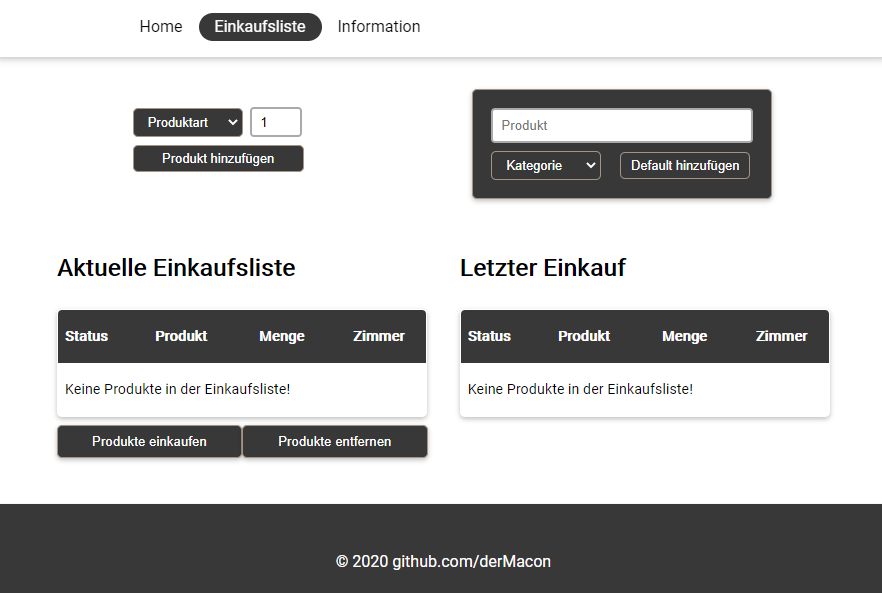
\includegraphics[width=.9\linewidth]{./_img/screenshot_01}
\end{figure}

\end{frame}






\begin{frame}{Roadmap}

Unmittelbar:
\begin{itemize}
\item Adminbereich einführen (neue Nutzer, etc.)
\item Darstellung aufräumen (Bootstrap, etc.)
\end{itemize}

Mittelfristig:
\begin{itemize}
\item Handyapp für Einkäufer
\begin{itemize}
\item REST Service notwendig (Client-Authentification)
\end{itemize}
\end{itemize}

Langfristig:
\begin{itemize}
\item Forum für Protokolle der WG-Treffen
\item Archiv über Stauräume im Haus
\end{itemize}

\end{frame}

  
\end{document}